\documentclass[10pt]{beamer}

\mode<presentation>
{
  \usetheme[height=1.25cm]{Madrid}
  \setbeamertemplate{navigation symbols}{}
  \setbeamercolor{alerted text}{fg=illini}
}
\usebackgroundtemplate{
\includegraphics[width=\paperwidth,height=\paperheight]{uc-background}}

\usepackage[english]{babel}
\usepackage{epsfig,subfigure,bm}
\usepackage{multimedia}
\usepackage{psfrag}
\usepackage{animate}

%%%%%% Begin of my macros and options

\setbeamertemplate{section in toc shaded}[default][55]
\setbeamertemplate{subsection in toc shaded}[default][55]
\setbeamercolor{block title}{fg=white,bg=illini}
\setbeamercolor{block body}{fg=black,bg=mygrey}

\setbeamercolor{emphprimary}{fg=CBlue}
\setbeamercolor{emphsecondary}{fg=illini}
\setbeamercolor{emphtertiary}{fg=mygreen}
\definecolor{darkForestGreen}{rgb}{.1,1,.1}
\definecolor{veryLightGray}{rgb}{.9,.9,.9}
\definecolor{greenApple}{rgb}{.3,.9,.3}

\setbeamercolor{frametitle}{bg=CBlue}   
\setbeamercolor{title}{bg=CBlue}

\usepackage{amsmath,amssymb,amsxtra,amsthm}
\usepackage{algorithm,algorithmic}
\usepackage{natbib}
\usepackage{bibentry}
\usepackage{xspace}
\usepackage{changepage}

\pdfmapfile{+sansmathaccent.map}

\definecolor{myblue}{rgb}{.2,.2,.7}
\definecolor{myred}{rgb}{.7,.2,.2}
\definecolor{mygreen}{rgb}{.2,.7,.2}
\definecolor{mygrey}{rgb}{0.9,0.9,0.9}
\definecolor{CBlue}{cmyk}{1,0.25,0,0}
\definecolor{illini}{rgb}{0.98,0.4,0.05}
\definecolor{black}{cmyk}{0,0,0,1}

\newcommand{\myemph}[1]{{\usebeamercolor[fg]{emphprimary}
    \textbf{#1}}}
\newcommand{\myemphalt}[1]{{\usebeamercolor[fg]{emphsecondary}
    \textbf{#1}}}

\graphicspath{{figs/}}

\title[Math for Robotics] % (optional, use only with long paper titles)
{CSE276C - Optimization}

\author[H.~I. Christensen] % (optional, use only with lots of authors)
{Henrik I.~Christensen}
% - Give the names in the same order as the appear in the paper.  -
% Use the \inst{?} command only if the authors have different
% affiliation.

\AtBeginSection[]
{
   \begin{frame}
       \frametitle{Outline}
       \tableofcontents[currentsection]
   \end{frame}
}

\institute[UCSD] % (optional, but mostly needed)
{
  \begin{minipage}[c]{.2\textwidth}
    
\includegraphics[width=.65\linewidth]{ucsealnew}%
  \end{minipage}%
  \begin{minipage}[c]{.6\textwidth}
    \small
%%    \begin{center}
      Computer Science and Engineering\\
      University of California, San Diego\\
      \myemph{\url{http://cri.ucsd.edu}}\\          
%%    \end{center}

  \end{minipage}
%%  \vspace*{1ex}
}
%% - Use the \inst command only if there are several affiliations.
%% - Keep it simple, no one is interested in your street address.

\bigskip

\date[Oct 2021]% (optional, should be abbreviation of conference name)
{\small%
  October 2021}

\begin{document}
  
\nobibliography{/Users/hic/Dropbox/bibliography/bib-file}
\bibliographystyle{plain}

\begin{frame}[plain]
  \titlepage
\end{frame}

\section{Introduction}

\begin{frame}
  \frametitle{Introduction}
  \begin{itemize}
  \item We have discussed approximation and root finding. We can
    leverage these methods to study optimization.
  \item Most of robotics is about optimization
  \item Best trajectory between two points
  \item Best fit of a model to a swarm of data
  \item Optimal coverage of an area for fire monitoring
  \item Energy efficient travel from San Diego to Hawaii by water
  \end{itemize}
\end{frame}

\begin{frame}
  \frametitle{Literature}
  \begin{itemize}
  \item Numerical Recipes: Chapter 10
  \item Numerical Renaissance: Chap 14-16. (Part III)
  \end{itemize}
\end{frame}

\begin{frame}
  \frametitle{Example 1}
  \begin{itemize}
  \item Optimization of trajectories at high speed
  \end{itemize}
\end{frame}

\begin{frame}
  \frametitle{Path Planning}
  \begin{itemize}
  \item Example potential field
    \centerline{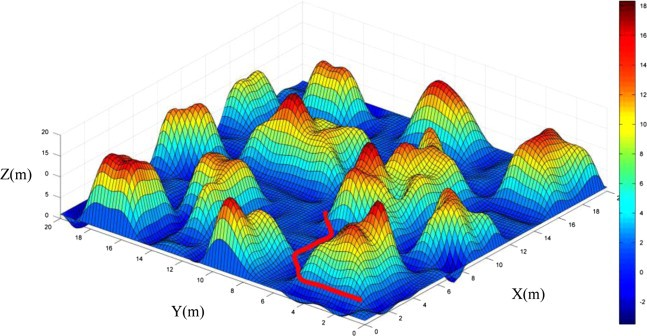
\includegraphics[height=5.5cm]{potential-field}}
  \end{itemize}
\end{frame}

\begin{frame}
  \frametitle{Optimization}
  \begin{itemize}
  \item So what is optimization? \pause
  \item Finding extrema for a function over a domain
  \item Minimum or maximum is immaterial as we can use f or -f
  \item In many cases we will have local and global extrema
  \item Consider both deterministic and stochastic approaches
  \end{itemize}
\end{frame}

\section{Bracket based methods}
\label{sec:golden-section}

\begin{frame}
  \frametitle{Golden section}
  \begin{itemize}
  \item For bracketing of roots we use bi-section as a basis. 
  \item We can use a similar technique to find an extremum
  \item We need two points to bracket a root!
  \item How many points do we need to bracket an extremum? \pause
  \item We need three points to bracket. 
  \item If we have a triplet $ a < b < c$. Iff f(b) is smaller than
    f(a) and f(c), then we have a minimum within $[a,c]$
  \end{itemize}
\end{frame}

\begin{frame}
  \frametitle{Golden Section}
  \begin{itemize}
  \item Pick a point between (a,b) or (b,c) and evaluate 
  \item Suppose $x\in (b,c)$ and $f(x) < f(b)$ then our new triple is
    (b, x, c)
  \item Consider the function
    \centerline{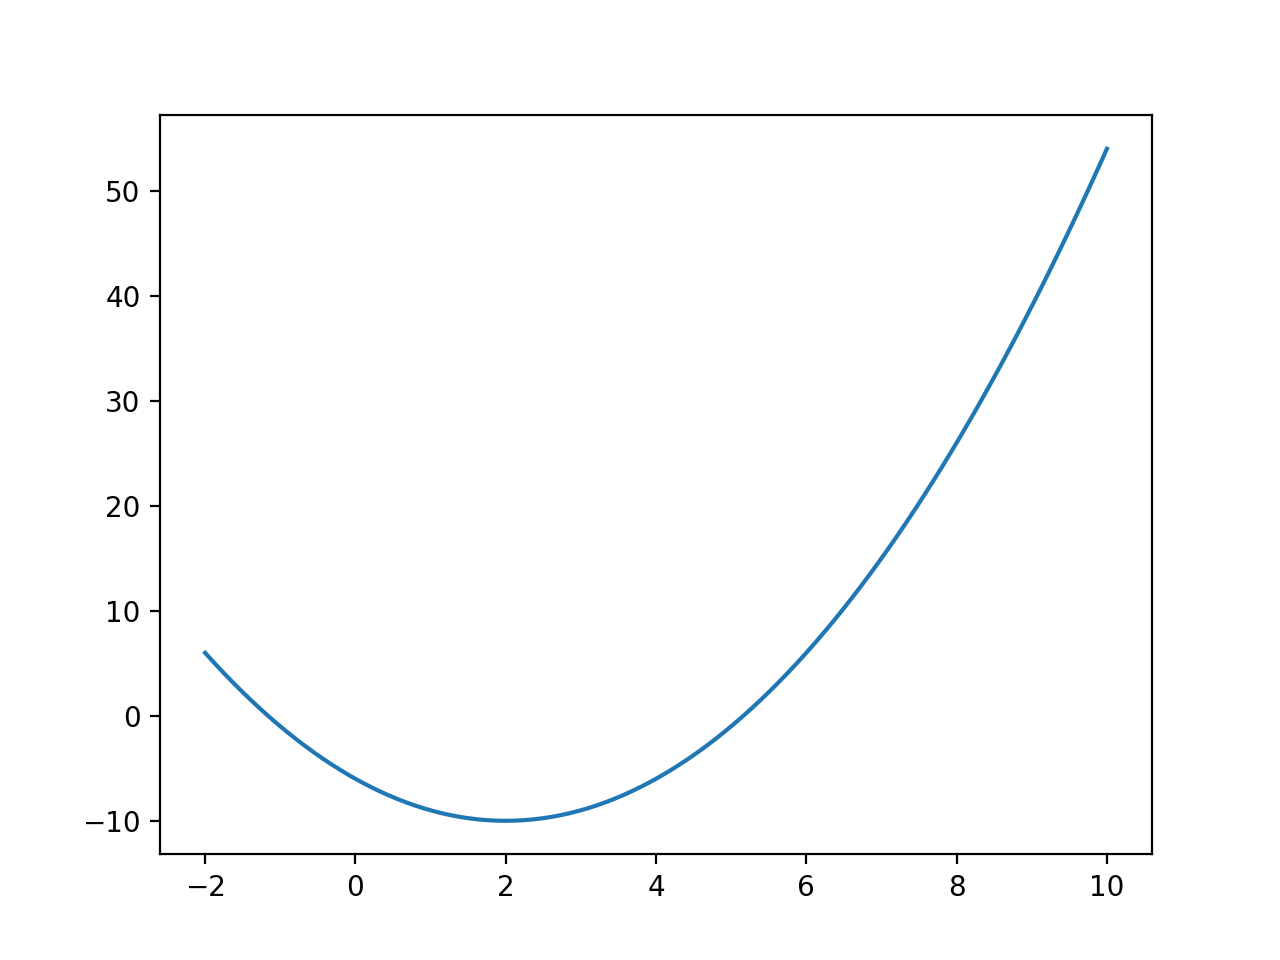
\includegraphics[height=5cm]{minimum}}
  \item How would you choose a new value of x? 
  \end{itemize}
\end{frame}

\begin{frame}
  \frametitle{Golden Section (cont.)}
  \begin{itemize}
  \item Consider (a, b, c)
    \[
      \begin{array}{ccc}
        \frac{b-a}{c-a} = w& ~~~~~ & \frac{c-b}{c-a} = 1-w\\
      \end{array}
    \]    
  \item Lets assume $x \in (b,c)$ and
    \[
      \frac{x-b}{c-a} = z
    \]
  \item The next bracket is then w+z or 1-w
    \pause
  \item If we want to make the intervals equal
    \[ z = 1-2w \mbox{~~~~~~ when } w < \frac{1}{2} \]
  \item z should be the same distance from b and c and b is from a and c
    \[ \frac{z}{1-w} = w \]
  \item we can rewrite to replace z and get the equation
    \[ w^2 - 3w +1 = 0 \Rightarrow w = \frac{3-\sqrt{5}}{2} \approx 0.38197 \]
  \item Widely used to select iteration strategies
  \end{itemize}
\end{frame}


\begin{frame}
  \frametitle{Parabolic Interpolation}
  \begin{itemize}
  \item We covered Brent's method in root finding and in interpolation
  \item If we have a triple (a, b, c) and the values f(a), f(b), f(c) we
    can generate a 2nd order interpolation
    \[
      x = b - \frac{1}{2} \frac{(b-a)^2 [f(b)-f(c)] - (b-c)^2 [f(b)-f(a)]}{(b-a)[f(b)-f(c)] - (b-c)[f(b)-f(a)]}
    \]    
  \item When would this fail?
    \pause    
  \item When the triple pair is co-linear!
  \item The remedy is to use golden section when a co-linear case is seen
  \end{itemize}
\end{frame}

\begin{frame}
  \frametitle{1-D search w. derivative information}
  \begin{itemize}
  \item If we have the triple (a, b, c) and f(a), f(b), f(c) 
  \item In addition we have f'(b)
  \item You can use the sign of f'(b) to choose the next bracket
  \end{itemize}
\end{frame}


\section{Downhill Simplex}
\label{sec:downhill-simplex}

\begin{frame}
  \frametitle{Simplex Method}
  \begin{itemize}
  \item Assume we have no gradient information or access to formal model. 
  \item A simplex is N dimensions is composed of N+1 points. Connected by
    straight lines
    \begin{itemize}
    \item A 2D simplex is a triangle
    \item A 3D simplex is a tetrahedron. 
    \end{itemize}
  \item We have N+1 points $x_1, \ldots, x_{N+1}$
  \end{itemize}
\end{frame}

\begin{frame}
  \frametitle{Downhill Simplex Algorithm}
  \begin{itemize}
  \item Initial simple
    \begin{itemize}
    \item Order the values of the vertices:
      $f(x_1) \leq f(x_2) \leq \ldots \leq f(x_{N+1})$
    \end{itemize}
    \item Compute $x_0$, the centroid of all points except $x_{N+1}$
    \item \myemph{Reflection} compute $x_r = x_0 + \alpha (x_0 - x_{N+1})$, with $\alpha>0$ if the reflection is better than $f(x_{N-1})$ replace. Restart
    \item \myemph{Expansion} if $f(x_r) < f(x_1)$ compute $x_e = x_0 + \gamma (x_r - x_0)$  if $f(x_e) < f(x_r)$ replace $x_{N+1}$ else replace $x_{N+1}$ with $x_r$. Restart
    \item \myemph{Contraction} If $f(x_r) > f(x_N)$ compute $x_c = x_0 + \rho (x_{N+1}  - x_0)$ with $\rho< .5$. If $f(x_c) < f(x_{N+1})$ replace and restart
    \item \myemph{Shrink} Replaces all points except $x_1$ with $x_i = x_1 + \sigma (x_i - x_1)$ and restart
    \item Terminate when update is below a threshold.
  \end{itemize}
\end{frame}

\begin{frame}
  \frametitle{Simplex illustration}
  \centerline{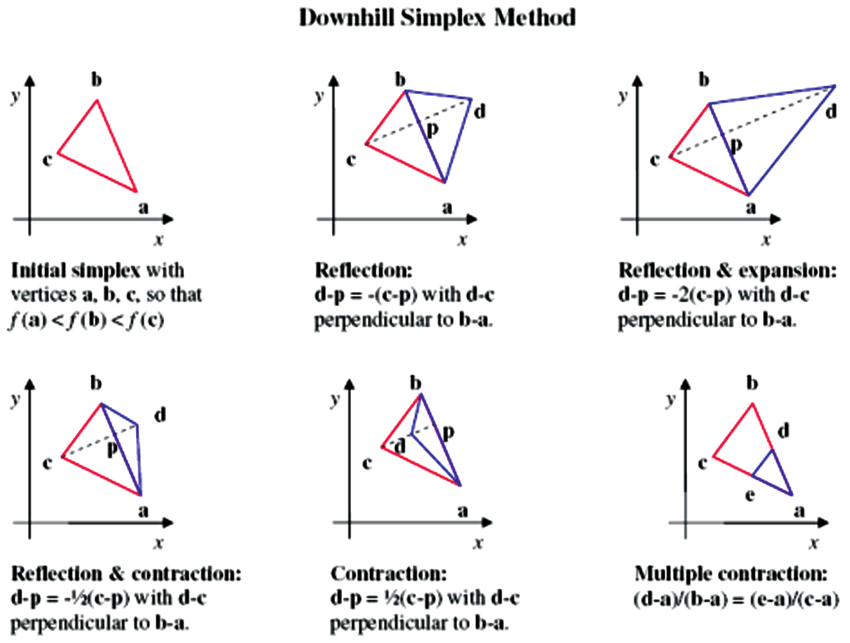
\includegraphics[height=7cm]{simplex}}
\end{frame}

\section{Powell's Method}
\label{sec:powells-method}

\begin{frame}
  \frametitle{Powell's Method}
  \begin{itemize}
  \item Assume you have an n-dimensional function $f(\vec{x})$ and a starting point $P_0$. 
  \item We can use the local gradient to search for an extremum
  \item We can generate a new estimate
    \[
      P_{new} = P_{old} + \lambda \vec{n}
    \]
  \item Locally we can generate a Taylor expansion
    \[
      f(x) = f(P) + \sum_i \frac{\partial f}{\partial x_i} x_i + \frac{1}{2} \sum_{ij} \frac{\partial^2f}{\partial x_i \partial x_j} x_i x_j + \ldots
    \] or 
    \[
      f(x) \approx \vec{c} - b \vec{x} + \frac{1}{2} \vec{x}^T A \vec{x}
    \] where
    \[
      \begin{array}{ccc}
        \vec{c} &= & f(P)\\
        b & = & - \nabla f_P \\
        A_{ij} & = & \frac{\partial^2 f}{\partial x_i \partial x_j} \mbox{~~ Hessian Matrix} \\
      \end{array}
    \] 
  \item Also remember
    \[ \nabla f = A x - b \]
    at an extremum
  \end{itemize}
\end{frame}

\begin{frame}
  \frametitle{Powell's Method}
  \begin{itemize}
  \item Initialize N unit vectors
    \[
      u_i = e_i \mbox{ ~~~ } i\in 1 ... N
    \]
    \begin{enumerate}
    \item Start at point $P_0$
    \item For i=1 to N
    \item \mbox{ ~~~ } Move along $P_i$ from $P_{i-1}$ along $u_i$
    \item \mbox{ ~~~ } New $u_i = u_{i+1}$
    \item \mbox{ ~~~ } Set $u_N = P_n - P_0$
    \item \mbox{ ~~~ } Move $P_n$ to minimum value 
    \item \mbox{ ~~~ } Make $P_0 = P_n$
    \end{enumerate}
  \item Might generate linear degenerate solutions
  \end{itemize}
\end{frame}

\section{Conjugate Descent/Gradient}
\label{sec:conj-desc}

\begin{frame}
  \frametitle{Conjugate gradient descent}
  \begin{itemize}
  \item If we have the gradient from
    \[
      f(x) \approx \vec{c} - b \vec{x} + \frac{1}{2} \vec{x}^T A \vec{x}
    \]
  \item We can do a steepest descent
    \begin{enumerate}
    \item Start at $P_0$
    \item Compute $\nabla f(P_i)$
    \item move in the direction of gradient to point $P_i$
    \item repeat
    \end{enumerate}
  \item We can construct a set of conjugate vectors
    \[
      \begin{array}{ccc}
        g_{i+1} & = & g_i - \lambda A h_i \\
        h_{i+1} & = & g_{i+1} + \gamma_i h_i\\
        \lambda_i & = & \frac{ g_i g_j }{ h_i A h_i }\\
        \gamma_i &=& \frac{g_{i+1} g_{i+1}}{ g_i g_i }\\
      \end{array}
    \]
  \end{itemize}
\end{frame}

\section{Stochastic Search}
\label{sec:stochastic-search}

\begin{frame}
  \frametitle{Stochastic Search}
  \begin{itemize}
  \item So far we have used direct functional values for optimization. 
  \item The search has been deterministic 
  \item Sometimes the search space is too large
  \item What if we use a sampling based approach?
  \item Some possible examples
    \begin{itemize}
    \item Traveling salesman
    \item Layout of silicon for chips
    \end{itemize}
  \item Loosely based on Boltzmann distribution
    \[
      P(E) = exp(-E/kT)
    \]
  \item where E is energy/entropy, T is temperature, and k is the
    Boltzmann constant.
    
  \end{itemize}
\end{frame}

\begin{frame}
  \frametitle{Metropolis Algorithm}
  \begin{itemize}
  \item Transformed into an algorithm by 1953 by Metropolis
  \item \myemph{Algorithm}
  \item Let $s= s_0$
  \item For $k=0 \mbox{ to } k_{max}$
    \begin{itemize}
    \item $T = temperature (k/k_{max}$
    \item Pick random neighbor $s_{new} = neighbor(T)$
    \item If $(P(S,T) \leq random(0,1)$
      \begin{itemize}
      \item $s = s_{new}$        
      \end{itemize}
    \end{itemize}
  \item Return S
  \end{itemize}
\end{frame}

\begin{frame}
  \frametitle{Simulated Annealing}
  \begin{enumerate}
  \item Description of possible configurations
  \item A way to generate random perturbation of a configuration
  \item An objective function whose minimization is the objective
  \item A control variable that is lowered over times. 
  \end{enumerate}
\end{frame}

\begin{frame}
  \frametitle{Example - traveling salesman}
  \begin{itemize}
  \item A salesman has to visit N cities at locations $(x_i, y_i)$
    returning to the original city
  \item Each city to be visited only once
  \item Minimize the travel route
  \item Problem in the optimal sense is known to be NP-hard. 
  \end{itemize}
\end{frame}

\begin{frame}
  \frametitle{Simple Example - Traveling Salesman}
  \centerline{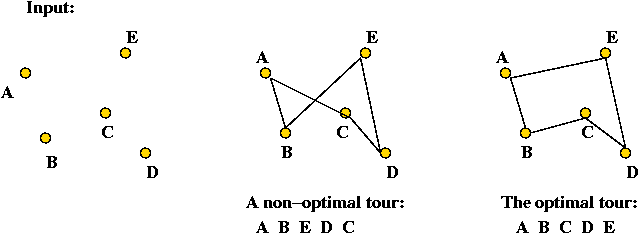
\includegraphics[width=10cm]{tsp}}
\end{frame}

\section{Dynamic Programming}
\label{sec:dynamic-programming}

\begin{frame}
  \frametitle{Dynamic Programming}
  \begin{itemize}
  \item So far we have considered functional optimization and
    stochastic optimization
  \item What if we have a limited set of action to optimize across? 
  \item Say optimizing a set of actions to traverse a graph? 
  \item A strategy to could be
    \begin{itemize}
    \item Generate a cost-map across the state space
    \item Backtrack to find the optimal set of actions
    \end{itemize}
  \end{itemize}
\end{frame}

\begin{frame}
  \frametitle{Dynamic programming}
  \begin{itemize}
  \item A number of different names / approaches has been used
    \begin{itemize}
    \item Bellman, Dijkstra, Viterbi, ... 
    \end{itemize}
  \item Selection a state space for optimization
  \item Identifying a set of possible actions
  \item Formulation of an objective function
  \end{itemize}
\end{frame}

\begin{frame}
  \frametitle{Example navigation}
  \centerline{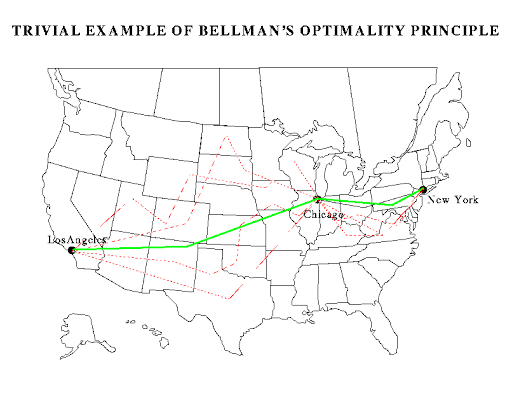
\includegraphics[height=6cm]{routing}}
\end{frame}


\begin{frame}
  \frametitle{Example navigation}
  \centerline{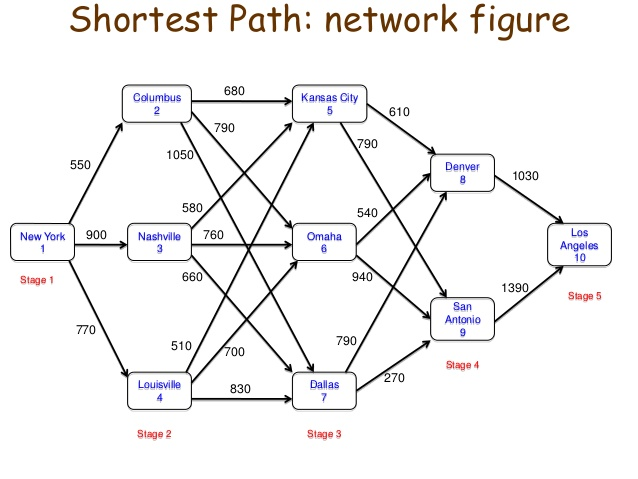
\includegraphics[height=6cm]{dynamic-programming-2}}
\end{frame}

\section{Summary}

\begin{frame}
  \frametitle{Summary}
  \begin{itemize}
  \item Optimization is a key objective in robotics
    \begin{itemize}
    \item Robotics is many cases is about formulation of a graph
    \item Optimization of an objective function across the graph
    \end{itemize}
  \item Considered deterministic and stochastic approaches to
    optimization
  \item Covered the basics and gave an impression of the fundamentals
  \end{itemize}
\end{frame}

\begin{frame}
  \frametitle{Questions}
  \centerline{\Huge Questions}
\end{frame}

\end{document}

%%% Local Variables:
%%% mode: latex
%%% TeX-master: t
%%% End:
